% allgem. Dokumentenformat
\documentclass[a4paper,12pt,headsepline]{scrartcl}
%Variablen welche innerhalb der gesamten Arbeit zur Verfügung stehen sollen
\newcommand{\titleDocument}{Bachelor- / Masterarbeit}
\newcommand{\subjectDocument}{im Studiengang <Studiengang>}

% weitere Pakete
% Grafiken aus PNG Dateien einbinden
\usepackage{graphicx}
\usepackage{scrextend}
\usepackage{gensymb}
\usepackage[numbers]{natbib}
\graphicspath{ {./img/methods/}{./img/results/}{./img/intro/}{./img/task/}{./img/procedure/}} 

% Eurozeichen einbinden
\usepackage[right]{eurosym}

% Umlaute unter UTF8 nutzen
\usepackage[utf8]{inputenc}

% Zeichenencoding
\usepackage[T1]{fontenc}

\usepackage{lmodern}
\usepackage{fix-cm}

% floatende Bilder ermöglichen
%\usepackage{floatflt}

% mehrseitige Tabellen ermöglichen
\usepackage{longtable}

% Unterstützung für Schriftarten
%\newcommand{\changefont}[3]{ 
%\fontfamily{#1} \fontseries{#2} \fontshape{#3} \selectfont}

% Packet für Seitenrandabständex und Einstellung für Seitenränder
\usepackage{geometry}
\geometry{left=3.5cm, right=2cm, top=2.5cm, bottom=2cm}

% Paket für Boxen im Text
\usepackage{fancybox}

% bricht lange URLs "schoen" um
\usepackage[hyphens,obeyspaces,spaces]{url}

% Paket für Textfarben
\usepackage{color}

% Mathematische Symbole importieren
\usepackage{amssymb}

% auf jeder Seite eine Überschrift (alt, zentriert)
%\pagestyle{headings}

% erzeugt Inhaltsverzeichnis mit Querverweisen zu den Kapiteln (PDF Version)
\usepackage[bookmarksnumbered,pdftitle={\titleDocument},hyperfootnotes=false]{hyperref} 
%\hypersetup{colorlinks, citecolor=red, linkcolor=blue, urlcolor=black}
%\hypersetup{colorlinks, citecolor=black, linkcolor= black, urlcolor=black}

% neue Kopfzeilen mit fancypaket
\usepackage{fancyhdr} %Paket laden
\pagestyle{fancy} %eigener Seitenstil
\fancyhf{} %alle Kopf- und Fußzeilenfelder bereinigen
\fancyhead[L]{\nouppercase{\leftmark}} %Kopfzeile links
\fancyhead[C]{} %zentrierte Kopfzeile
\fancyhead[R]{\thepage} %Kopfzeile rechts
\renewcommand{\headrulewidth}{0.4pt} %obere Trennlinie
%\fancyfoot[C]{\thepage} %Seitennummer
%\renewcommand{\footrulewidth}{0.4pt} %untere Trennlinie

% für Tabellen
\usepackage{array}

% Runde Klammern für Zitate
%\usepackage[numbers,round]{natbib}

% Festlegung Art der Zitierung - Havardmethode: Abkuerzung Autor + Jahr

% Schaltet den zusätzlichen Zwischenraum ab, den LaTeX normalerweise nach einem Satzzeichen einfügt.
\frenchspacing

% Paket für Zeilenabstand
\usepackage{setspace}

% für Bildbezeichner
\usepackage{capt-of}

% für Stichwortverzeichnis
\usepackage{makeidx}

% für Listings
\usepackage{listings}
\lstset{numbers=left, numberstyle=\tiny, numbersep=5pt, keywordstyle=\color{black}\bfseries, stringstyle=\ttfamily,showstringspaces=false,basicstyle=\footnotesize,captionpos=b}
\lstset{language=java}

% Indexerstellung
\makeindex

% Abkürzungsverzeichnis
\usepackage[german]{nomencl}
\let\abbrev\nomenclature

% Abkürzungsverzeichnis LiveTex Version
\renewcommand{\nomname}{Abkürzungsverzeichnis}
\setlength{\nomlabelwidth}{.25\hsize}
\renewcommand{\nomlabel}[1]{#1 \dotfill}
\setlength{\nomitemsep}{-\parsep}
\makenomenclature
%\makeglossary

% Abkürzungsverzeichnis TeTEX Version
% \usepackage[german]{nomencl}
% \makenomenclature
% %\makeglossary
% \renewcommand{\nomname}{Abkürzungsverzeichnis}
% \setlength{\nomlabelwidth}{.25\hsize}
% \renewcommand{\nomlabel}[1]{#1 \dotfill}
% \setlength{\nomitemsep}{-\parsep}

% Disable single lines at the start of a paragraph (Schusterjungen)
\clubpenalty = 10000
% Disable single lines at the end of a paragraph (Hurenkinder)
\widowpenalty = 10000
\displaywidowpenalty = 10000

\begin{document}
% hier werden die Trennvorschläge inkludiert
%hier müssen alle Wörter rein, welche Latex von sich auch nicht korrekt trennt bzw. bei denen man die genaue Trennung vorgeben möchte
\hyphenation{
Film-pro-du-zen-ten
Lux-em-burg
Soft-ware-bau-steins
zeit-in-ten-siv
}

%Schriftart Helvetica
%\changefont{phv}{m}{n}


% Titelseite %
% das Papierformat zuerst
%\documentclass[a4paper, 11pt]{article}

% deutsche Silbentrennung
%\usepackage[ngerman]{babel}

% wegen deutschen Umlauten
%\usepackage[ansinew]{inputenc}

% hier beginnt das Dokument
%\begin{document}


\thispagestyle{empty}

%\begin{figure}[t]
% \includegraphics[width=0.6\textwidth]{abb/fh_koeln_logo}
%\end{figure}


\begin{verbatim}


\end{verbatim}

\begin{center}
\Large{Universität Tübingen}\\
\Large{- Mathematisch-Naturwissenschaftliche Fakultät -}\\
\end{center}


\begin{center}
\Large{Externes Laborpraktikum}
\end{center}
\begin{verbatim}




\end{verbatim}
\begin{center}
\doublespacing
\textbf{\LARGE{Affordance Judgements in Virtual Reality}}\\
\singlespacing
\begin{verbatim}

\end{verbatim}
\textbf{im Studiengang Kognitionswissenschaft}
\end{center}
\begin{verbatim}

\end{verbatim}
\begin{center}

\end{center}
\begin{verbatim}

\end{verbatim}
\begin{center}
\textbf{}
\end{center}
\begin{verbatim}






\end{verbatim}
\begin{flushleft}
\begin{tabular}{llll}
\textbf{Autor:} & & Marcel Bechtold& \\
& & MatNr. 3949100 & \\
& & \\
\textbf{Version vom:} & & \today &\\
& & \\
\textbf{1. Betreuerin:} & & Prof. Dr. Martin Butz &\\
\textbf{2. Betreuer:} & & Dr. Betty Mohler &\\
\end{tabular}
\end{flushleft}

% römische Numerierung
%\pagenumbering{arabic}

% 1.5 facher Zeilenabstand
\onehalfspacing

% einfacher Zeilenabstand
\singlespacing

% Inhaltsverzeichnis anzeigen
\newpage
\tableofcontents

\newpage

% das Abbildungsverzeichnis
%\newpage
% Abbildungsverzeichnis soll im Inhaltsverzeichnis auftauchen
\addcontentsline{toc}{section}{List of Figures}
% Abbildungsverzeichnis endgueltig anzeigen
\listoffigures

% das Tabellenverzeichnis
%\newpage
% Abbildungsverzeichnis soll im Inhaltsverzeichnis auftauchen
\addcontentsline{toc}{section}{List of Tables}
% \fancyhead[L]{Abbildungsverzeichnis / Abkürzungsverzeichnis} %Kopfzeile links
% Abbildungsverzeichnis endgueltig anzeigen
\listoftables

% Definiert Stegbreite bei zweispaltigem Layout
\setlength{\columnsep}{25pt}

%%%%%%% EINLEITUNG %%%%%%%%%%%%
%\twocolumn
\newpage
\fancyhead[L]{\nouppercase{\leftmark}} %Kopfzeile links

% 1,5 facher Zeilenabstand
\onehalfspacing

% einzelne Kapitel
\newpage
\section{Introduction} \label{sec:introduction}

The goal of the internship is to learn how to implement and run Virtual Reality experiments. An existing experiment (Reaching Study) will be used to learn how to set up and run participants. Depending on how much time will be left two more follow-up experiments can be implemented and run during the internship.

In the virtual environment of the Reaching Study the participants find themselves sitting at a round table. Their task is to judge if they can reach for an object that appears on that table at different distances. Besides from their own perspective at the table most of the trials demand the participant to imagine to sit at a different location around the table. The question being addressed here is if the participants show different reaction times for different locations around the table which would argue for some kind of “mental rotation of the self in 3D”. Furthermore the data of these trials will provide the participants estimated maximum reaching distance. 
In the second part of the experiment the participant can actually reach for several objects on the table with a virtual arm controlled by the participant’s actual arm which is tracked by a controller. The virtual arm for one half of the participants is (20%) shorter and the other half (20%) longer than their actual arm.  
In the third part of the experiment the participants do the same task as in the first part. The question being addressed now is if the experience of a shorter/longer arm has the effect that the estimated maximum reaching distance is decreased/increased. This would support the idea that temporarily changing one’s body (and therefore one’s action capabilities) also changes perception. After having experienced a shorter (longer) arm, we argue the participants scale the object distance based on the new so called perceptual ruler which makes them perceive objects further away (closer). And as a result the estimated maximum reaching distance decreases (increases).
\newpage
\section{Methods}

\subsection{Participants}
37 participants(21 female, 16 male; all right-handed) from the local university community participated in the experiment. Their age ranged from 21 to 41 years. All participants were naive to the purpose of the experiment and had normal or corrected-to-normal vision. The experiment was approved by the ethics committee of the University of T\"ubingen, and was performed in accordance with the Declaration of Helsinki. Participants gave written informed consent prior to the experiment and were compensated with 8 Euro per hour for their participation. 

\subsection{Apparatus}
The virtual environment was displayed in stereo using an HTC Vive head-mounted-display (HMD) with a resolution of 1080 x 1200 pixels per eye (2160 x 1200 pixels combined). Inter-pupillary distance was measured with a pupilometer and set accordingly on the HTC Vive for each participant. Before the experiment two HTC Vive controllers were used to calibrate the experiment according to the participant's arm span. During the experiment one HTC Vive controller was attached to the participant's wrist to track hand and arm movements. The tracked controller movement data was used to display a virtual arm that moves according to the participants real movements. Participants were sitting during the whole experiment and viewed their virtual task in front of them. An XBox controller \ref{fig:xbox} was used in order to allow participants to make decisions and proceed to the next trial.

\begin{figure}
\centering
  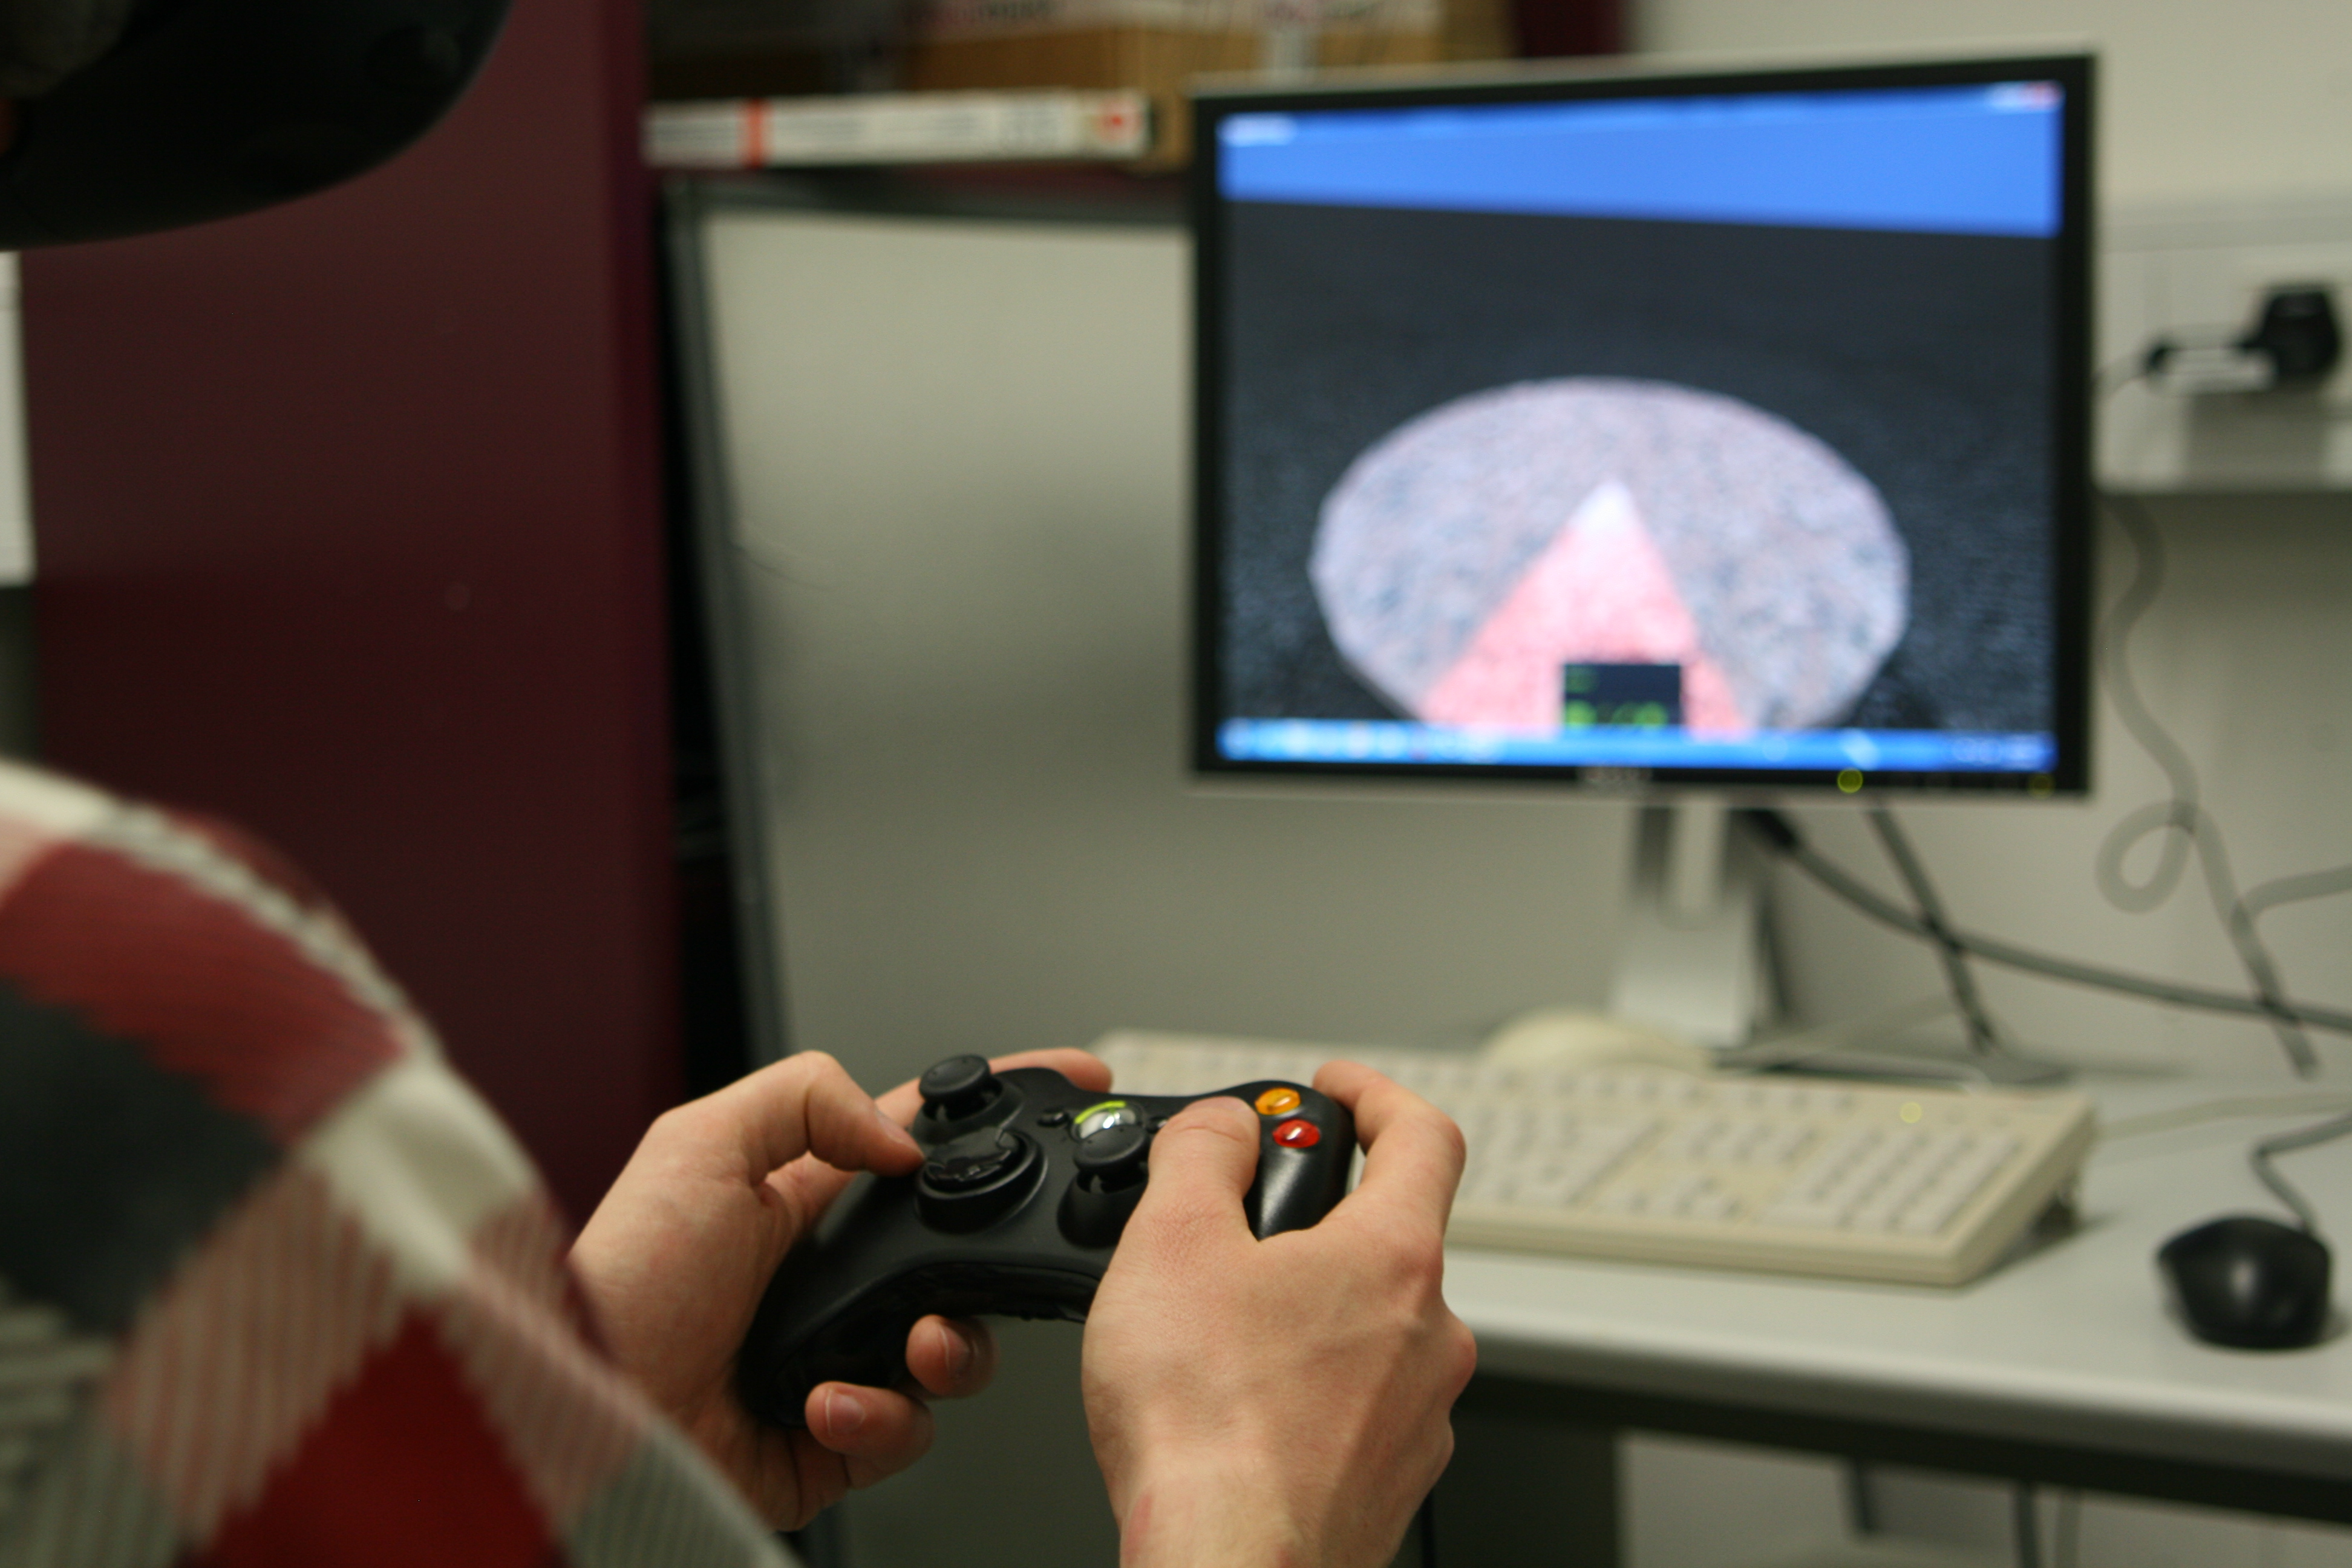
\includegraphics[width=0.5\textwidth]{xbox}
  \caption{XBox controller used to make decisions in the trial phase.} 
  \label{fig:xbox}
\end{figure}

In one part of the experiment (trial phase) the virtual environment consists of a round table and an empty chair which is located at the table and a small blue ball is located on top of the table. In the other part of the experiment (adaptation phase) the virtual environment consists of a square table an there a three different blue objects (a ball, a square and a capsule) located on top of the table. \ref{fig:trial_table}

\begin{figure}
\centering
  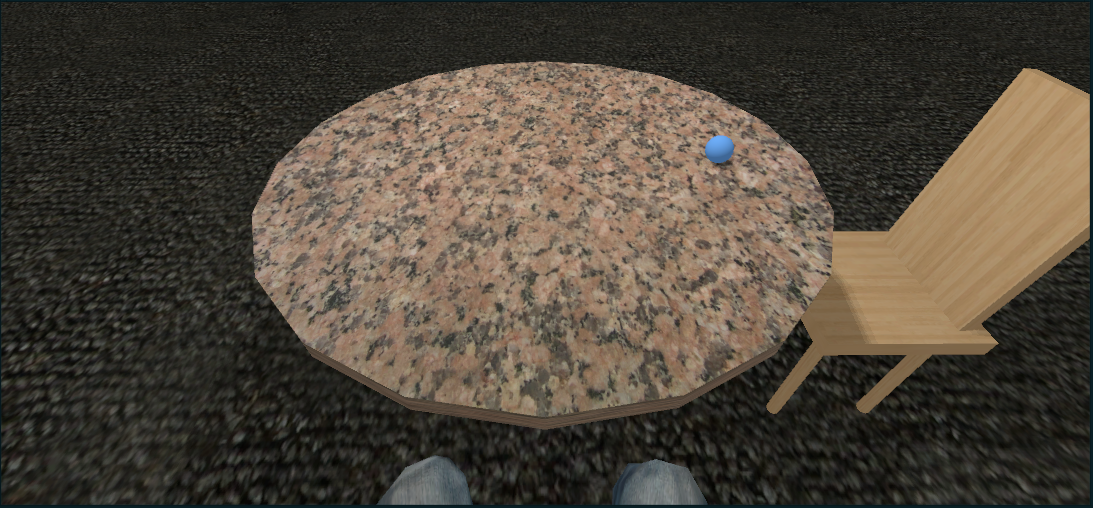
\includegraphics[width=0.5\textwidth]{trial_table}
  \caption{Virtual environment: table with ball and empty chair.} 
  \label{fig:trial_table}
\end{figure}


In the trial phase participants make a decision if they can reach the blue ball by pressing the shoulder buttons of the XBox Controller. The left shoulder button is used to decide that they can not reach the ball and the right shoulder button is used to decide they can reach it. Participants can start each trial by pressing the 'A' button of the XBox controller. In the adaptation phase participants only use their own hand movements to control their virtual arm which is tracked by the HTC Vive controller.

\subsection{Procedure}
The experimenter explained the details of the experiment to each participant before the experiment. Participants will perform a virtual reality task and will wear a head mounted display during the entire experiment. They will sit during the entire experiment and see a round virtual table in front of them. The task will be to judge if they can reach an object that appears on different locations on the table. It is important for the participants to imagine that they can not lean forward to reach the object. Furthermore it is important to make the decision imagining to sit on a chair that appears on different locations around the table for each trial. And sometimes that chair will have their actual location. The usage of the XBox controller was explained like in the section Apparatus. Finally participants were informed that later during the experiment HTC Vive controllers will be used to track their hand movements.

The whole experiment consists of two trial phases and one adaptation phase between the trial phases.

Each trial phase consists of 336 Trials. One trial is to judge if the participant would be able to reach the ball on the table and consists of two steps. First, a red light on the table indicates where an empty chair will appear. The participant confirms the light indicator using the XBox controller. Second, the empty chair appears and the participant decides also via XBox controller if he or she would be able to reach the ball.

In the adaptation phase participants can interact with objects on a square table in a virtual environment similar to the one in the trial phase. In preparation of the adaptation phase the distance between the participants wrists sitting in a T-position is measured. \ref{fig:controller_calibration} The measurement is used as an input variable for the virtual environment to visualize the participant's arm length. There are two conditions. One group of participants will see a representation of their arm that is only 80\% of their actual arm length and the other group of participants will see a representation of their arm that is 120\% of their actual arm length. In order to control their virtual arm a controller will be attached to the writs of the dominant arm of the participant. \ref{fig:controller_attach} Therefore the virtual arm can mirror the actual movements of the participant. The task in the adaptaion phase is to reach out to 3 objects on the table. The objects disappear if the participant is able to reach them and they remain on the table if the participant is not able to reach them. Participant's are not allowed forward to reach the objects. There 20 repetitions with 3 objects each. \ref{fig:controller_use}

\begin{figure}[h]
\centering
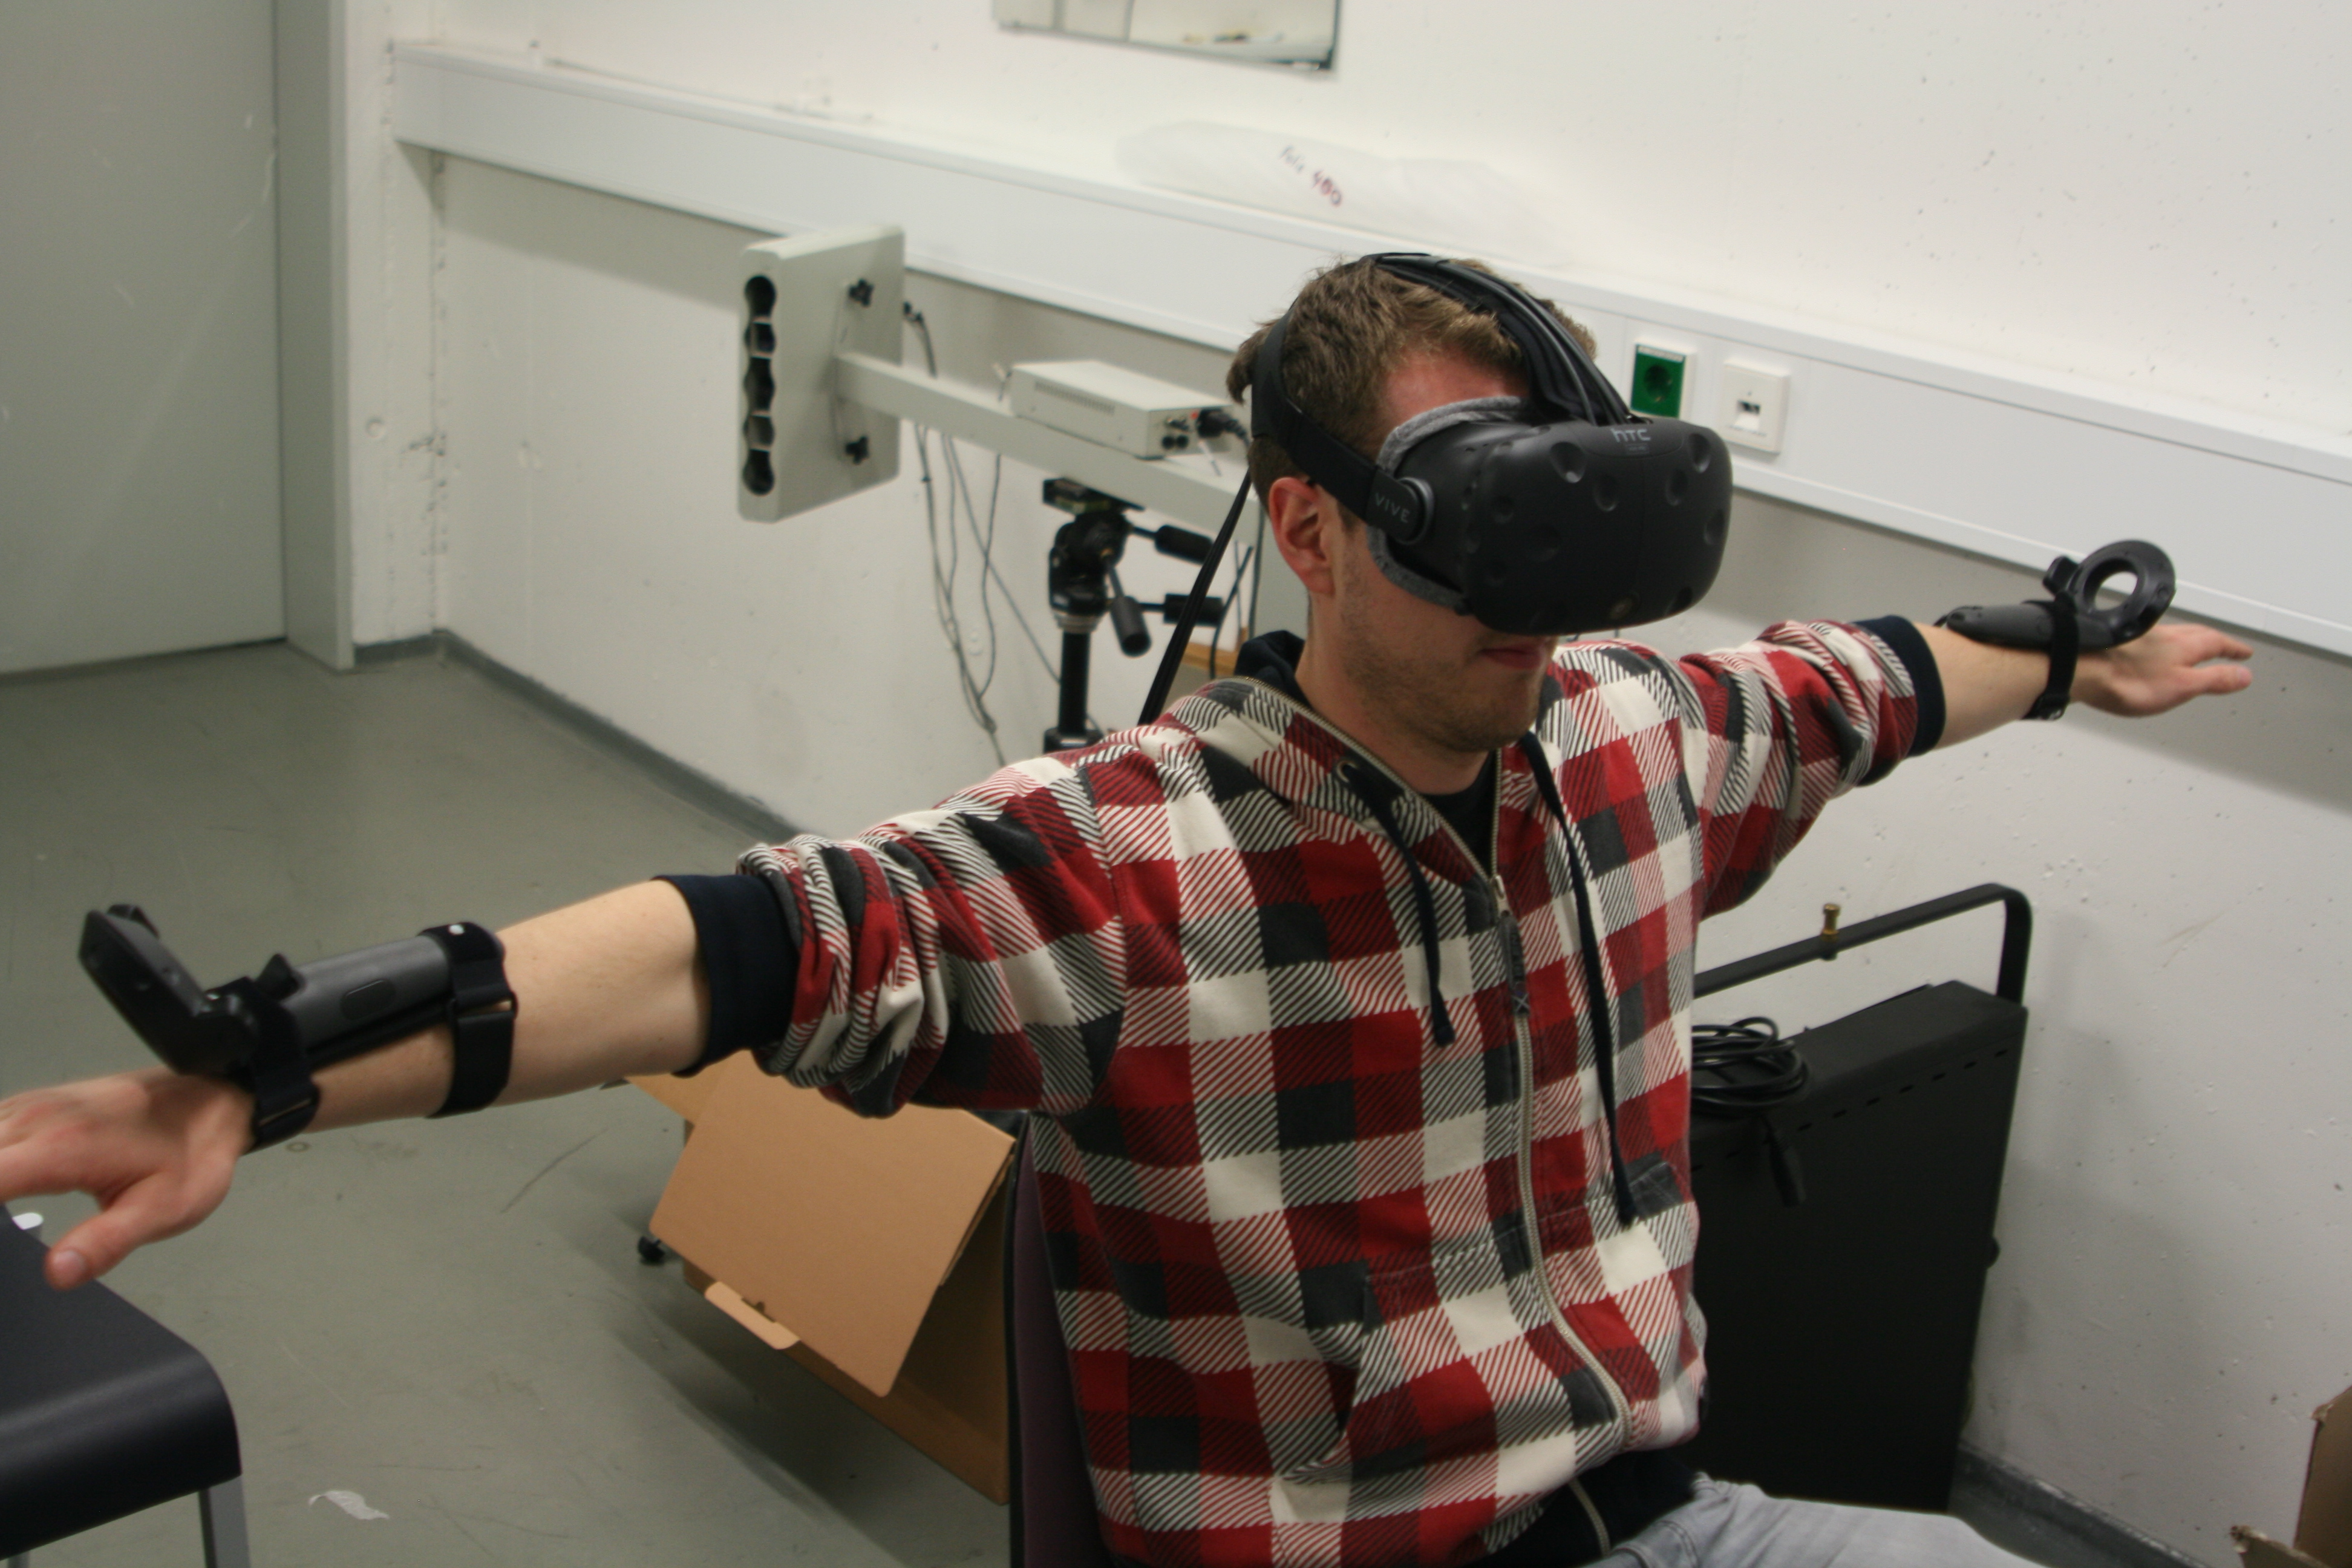
\includegraphics[width=0.5\textwidth]{controller_calibration}
\caption{Two HTC Vive controller attached to the participant's arms to measure and calibrate the virtual arm.}
\label{fig:controller_use}
\end{figure}

\begin{figure}[h]
\centering
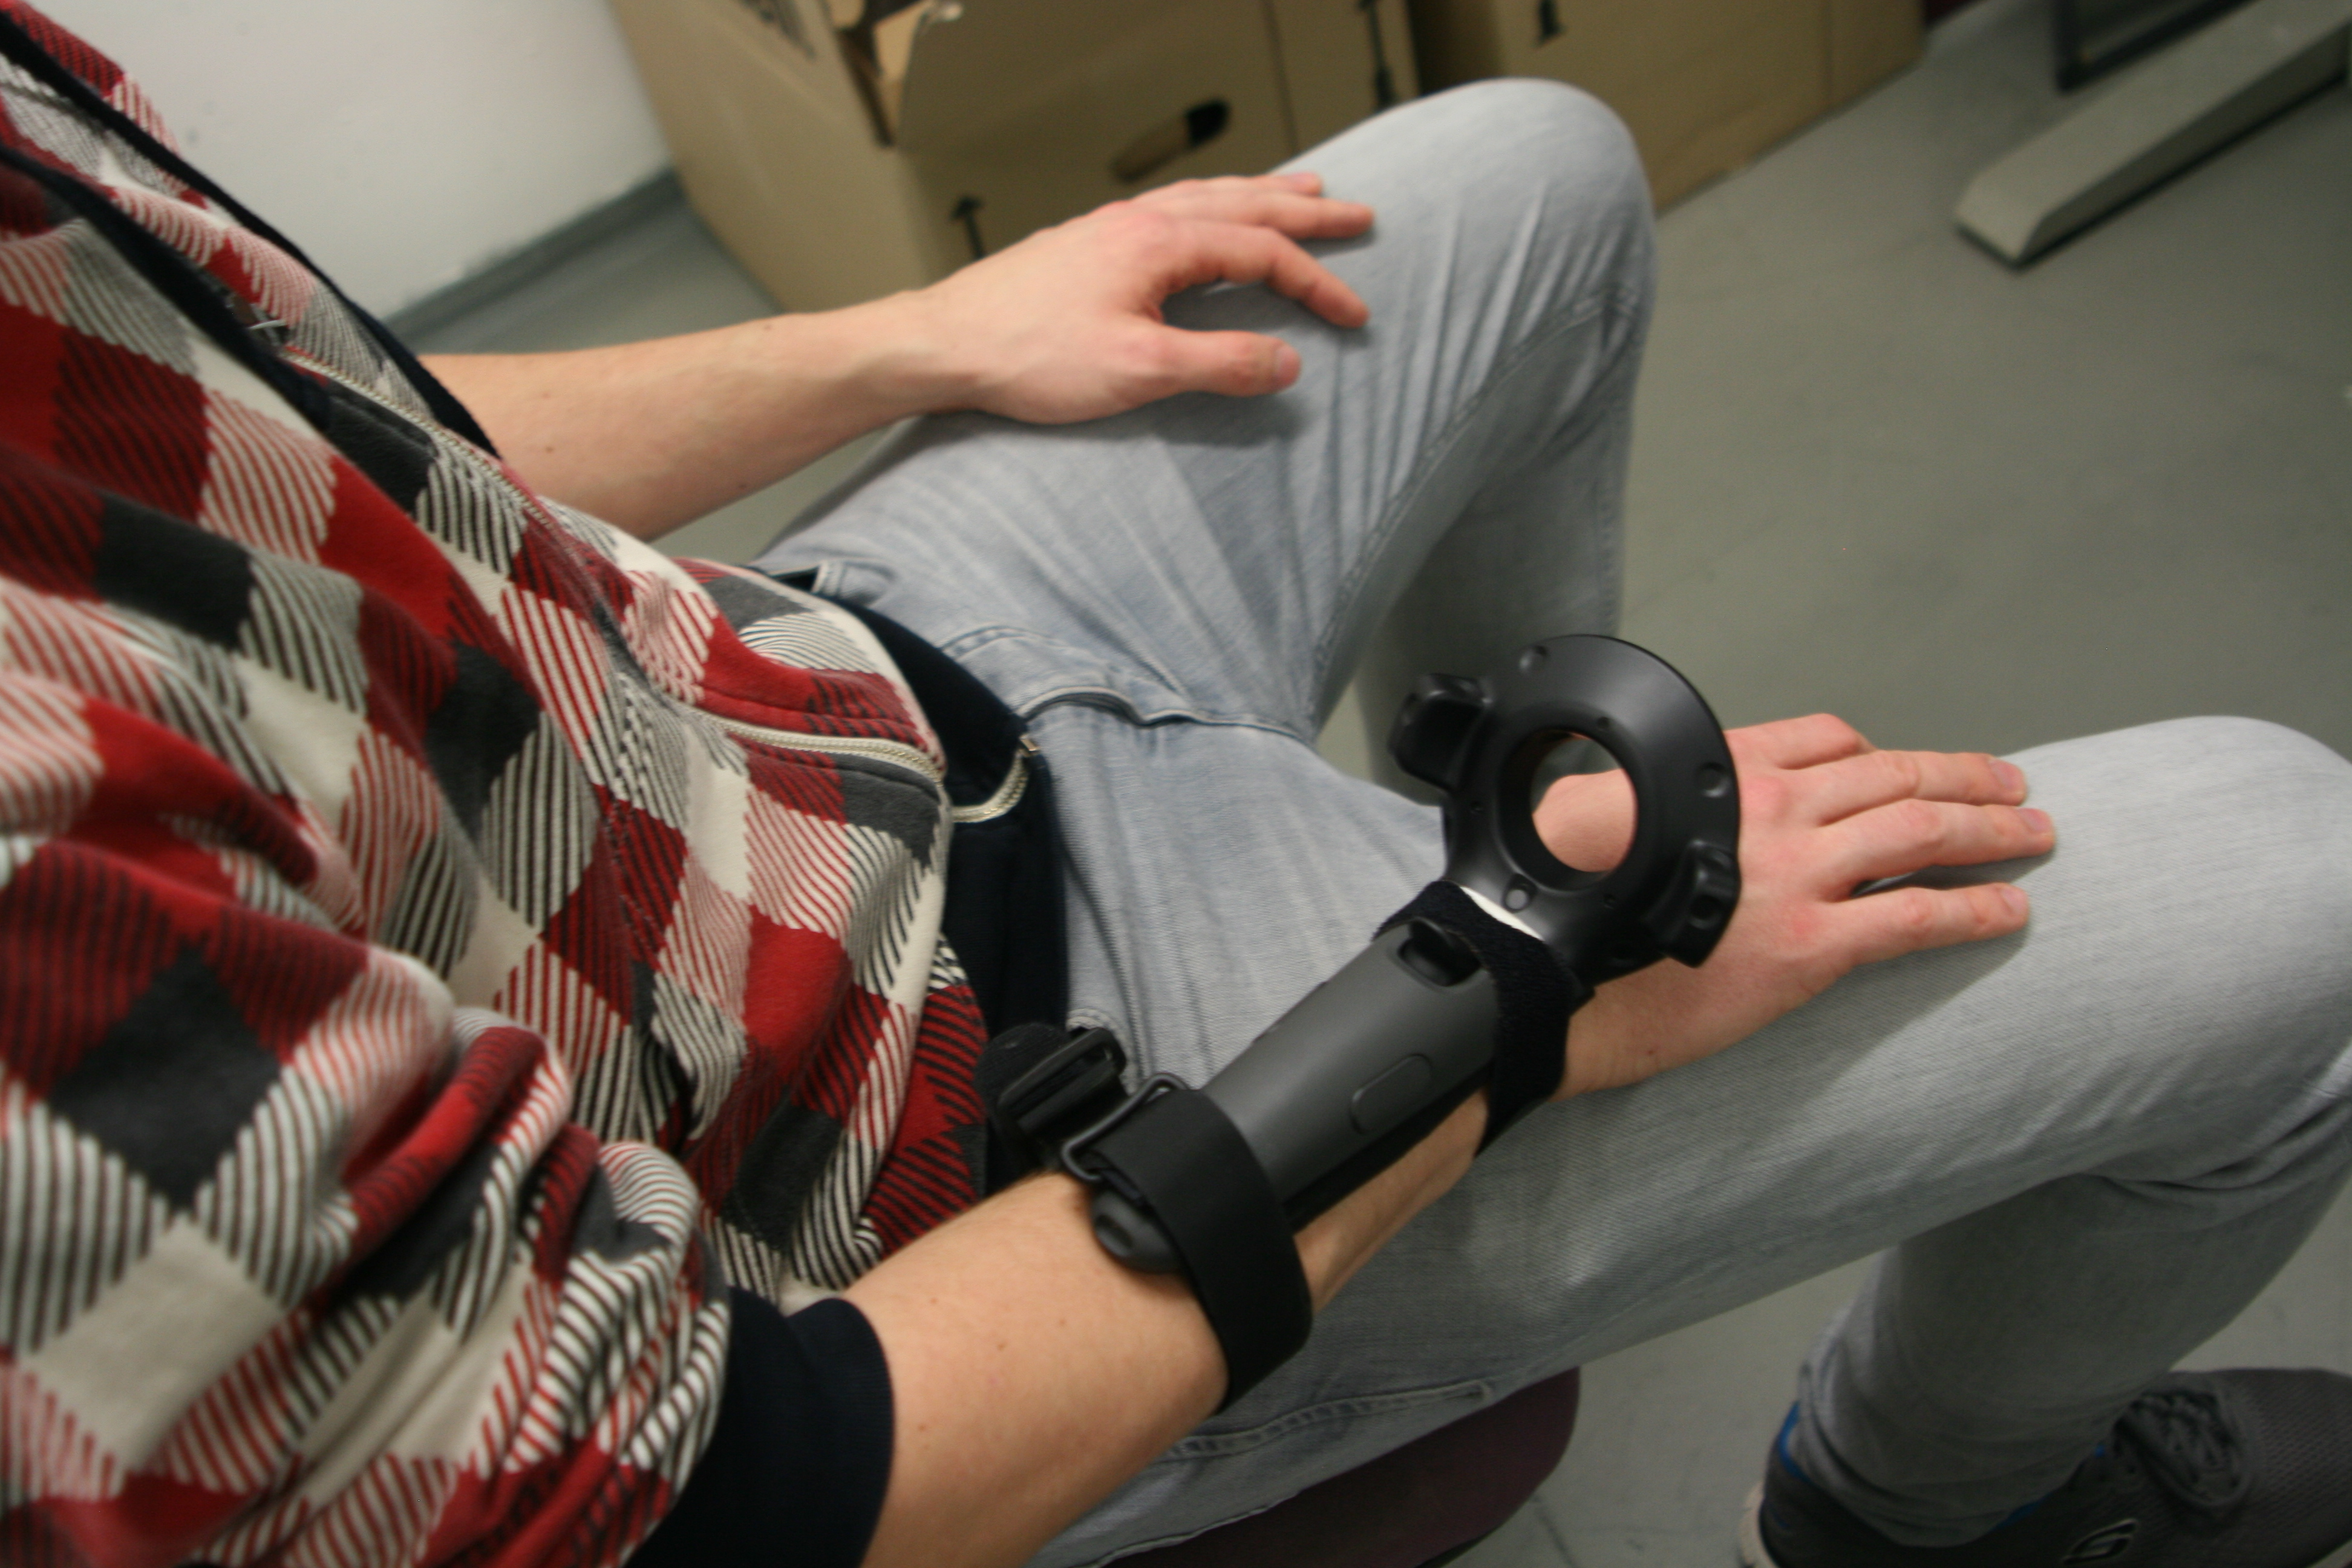
\includegraphics[width=0.5\textwidth]{controller_attach}
\caption{HTC Vive controller attached to the participant's arm to track hand and arm movements.}
\label{fig:controller_calibration}
\end{figure}

\begin{figure}
\centering
  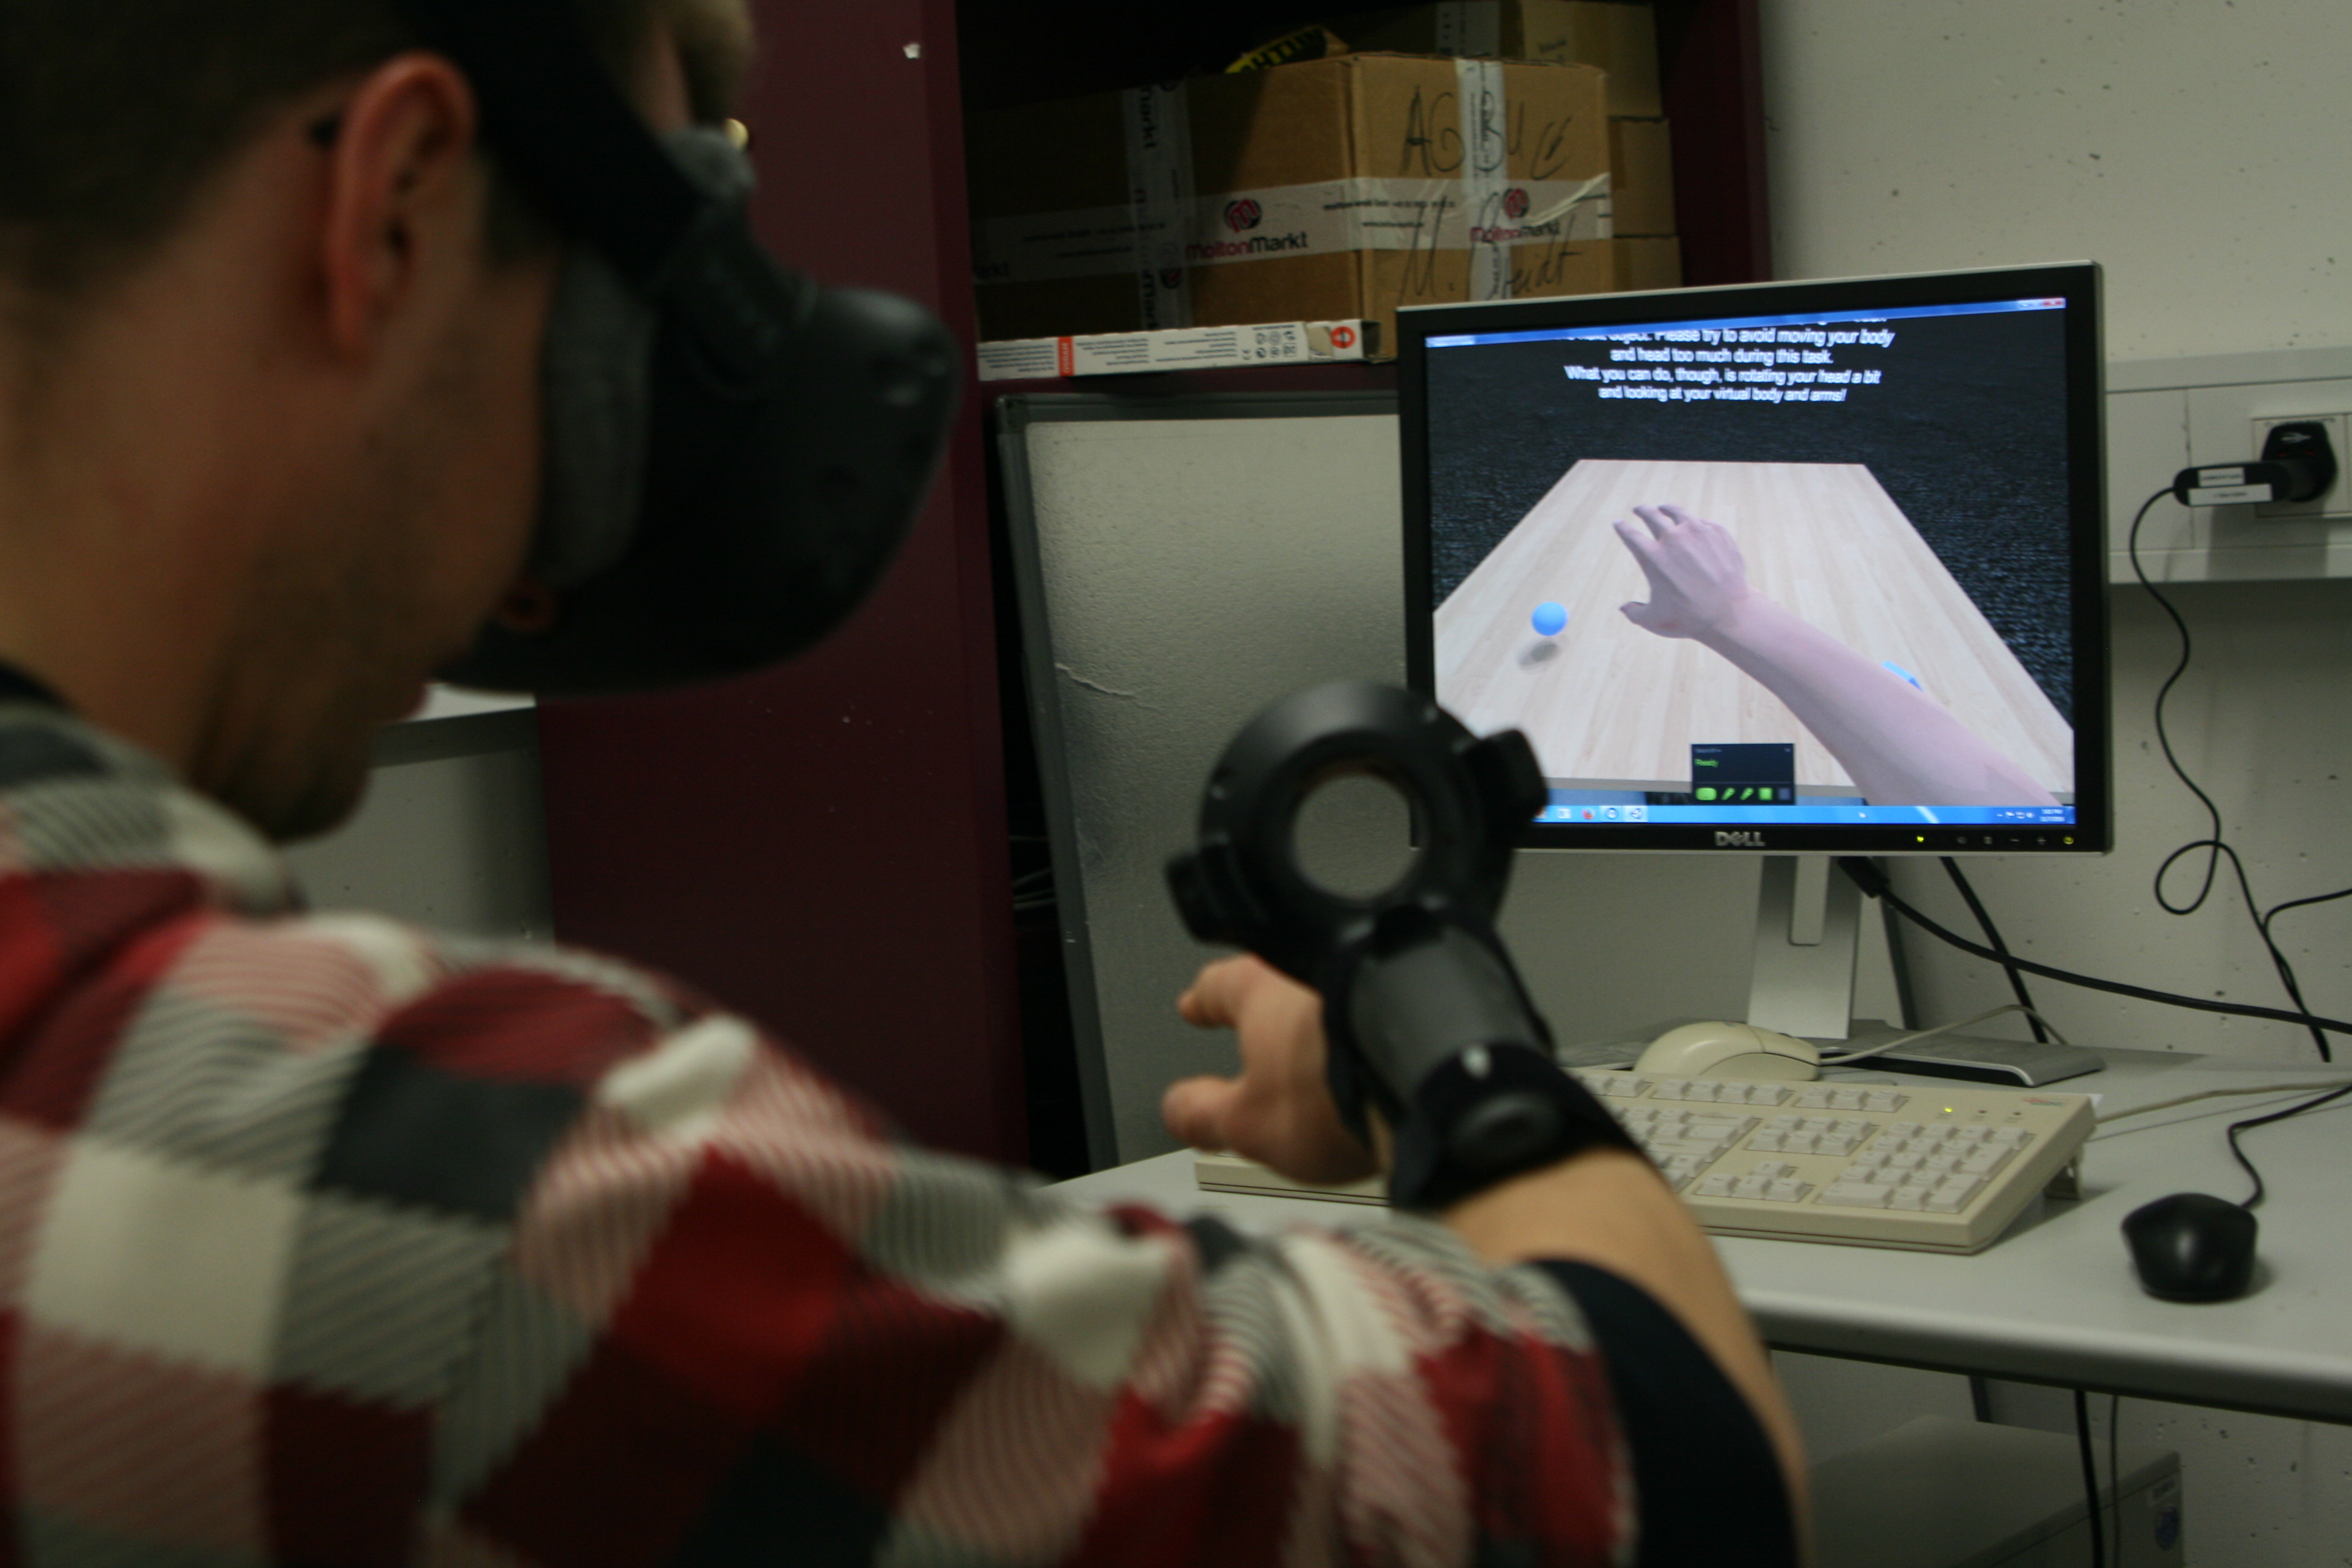
\includegraphics[width=0.5\textwidth]{controller_use}
  \caption{HTC Vive controller attached to the participant's arm to track hand and arm movements.}
  \label{fig:controller_attach}
\end{figure}



%what needs to go in here is:

%instructions that were given to the participants
%training phase (how many trials...)
%counterbalance single / multi (counterbalanced - 10 each side)

\newpage
\section{Results and Discussion}

Response times and accuracy was considered for analysis. Accuracy was calculated as the ratio of estimated to actual reach. Estimated maximum reach was determined by the crossover point from yes to no responses. (Fig. \ref{fig:cross_over}) The actual reach was measured after the experiment. A crossover point greater than 1 means over estimation, a crossover point smaller than 1 means under estimation. 

\begin{figure}
\centering
  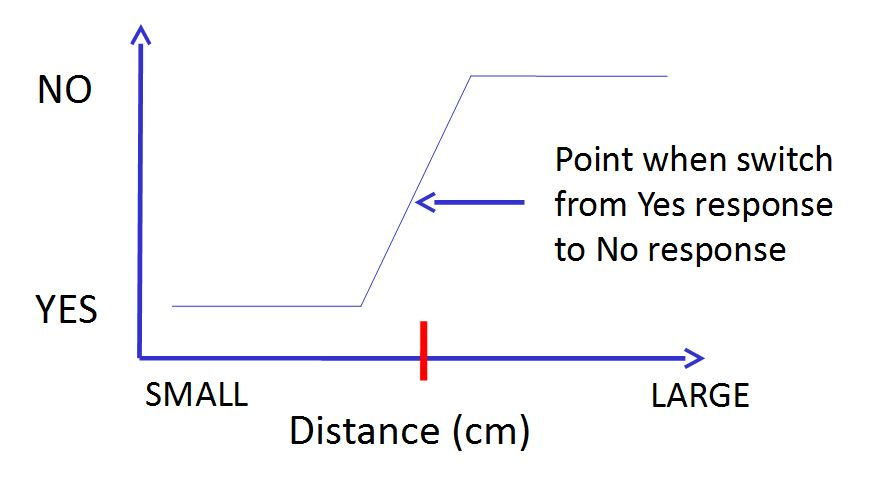
\includegraphics[width=0.75\textwidth]{cross_over}
  \caption{Crossover point: ratio of estimated reach to actual reach.} 
  \label{fig:cross_over}
\end{figure}

\subsection{Response Time}

Firstly, response time did not significantly increase with a greater rotation of the chair. This is not inline with our hypothesis that participants show different reaction times for different locations around the table. Therefore we conclude that there is no cost in reaction time because of “mental rotation of the self in 3D”. An explanation for the consistent reaction times for different rotations could be a visual heuristic used by participants. It is possible that participants imagine a circle on the table which indicates how far they assume they are able to reach. This would make it unnecessary to actively rotate oneself to the target location so that reaction times are independent from the angle of the rotation.

Secondly, as shown in Fig. \ref{fig:no_arm_responst_time_dist} response times in the no arm condition were overall higher than in the shorter/longer arm condition. Since the no arm condition was always the first of the two trial phases this result could be caused by a training effect. Participants were less experienced with the task and therefore required more time to respond. Furthermore they have not yet had any control over their virtual arm so that their judgment is solely based on their imagination.  After having controlled their virtual arm in the adaptation phase, participants get a better understanding of how far they can reach in the second trial phase. This could also cause shorter reaction times in the second trial phase (shorter or longer arm condition).

\begin{figure}
\centering
  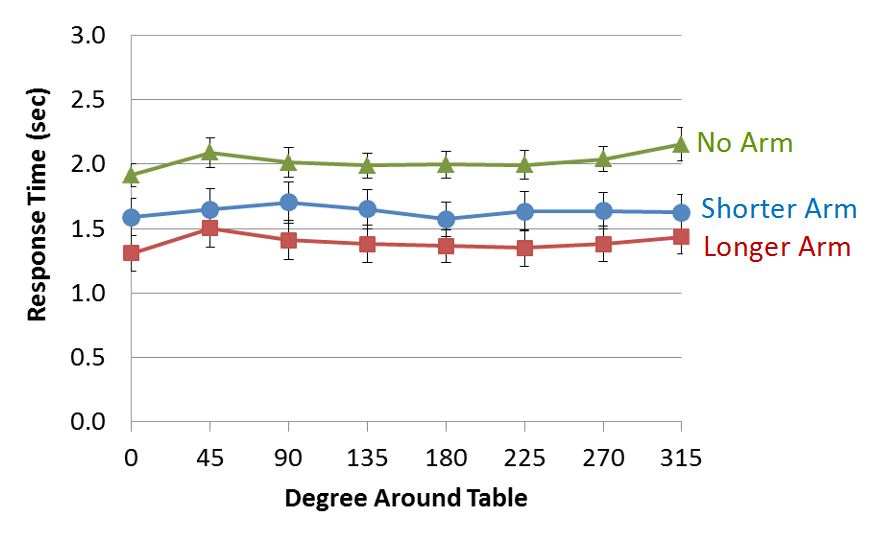
\includegraphics[width=0.75\textwidth]{all_response_time}
  \caption{Response times of different chair angles around the table in all conditions} 
  \label{fig:all_response_time}
\end{figure}

For each condition there is a clear peak of response times in relation to a specific distance of the ball from the edge of the table. The overall shape of the graph can be described as an upside down 'v' and therefore showing lower response times the shorter and higher distances get. In the no arm condition the peak is at 45 cm from the edge of the table with a response time of 2.5 seconds. (Fig \ref{fig:no_arm_responst_time_dist}) The peak response times in this graph indicate that it was the most difficult to make a judgment at a certain distance from the edge of the table. We assume that this distance must be very close to the participant's estimated maximum reaching distance. The closer the ball is to the participant's maximum reaching distance the more difficult it is to make a decision, because a yes and no response become equally likely.
Looking at shorter and higher distances one can observe the opposite effect of lower response times. Since it is obvious that an object can be reached when it is very near (or can not be reached when it is very far) it also easier to make a decision which results in lower response times. 

In the shorter arm condition the peak is at 30 cm from the edge of the table with a response time of 2.1 seconds. And in the longer arm condition the peak is at 40 cm with a response time of 1.7 seconds. (Fig \ref{fig:short_long_arm_responst_time_dist}) Expectedly, in the shorter arm condition participants show a peak reaction time at a shorter distance of the ball from the edge of the table than in the longer arm condition. Thus, having perceived and controlled their virtual arm not only results in shorter reaction times. It also affects the estimated maximum reaching distance. Having Perceived and controlled a shorter arm causes participants to experience a shorter maximum reaching distance and vise versa. 

Comparing the distances of shorter/longer arm condition at peak reaction times (30cm and 40cm) with the no arm condition it is interesting to observe that both the distances of shorter and longer arm condition are smaller than in the no arm condition (45cm). Without the data provided in the experiment one would probably assume that the distances must be higher for the the longer arm condition and smaller for the shorter arm condition. A general explanation for this effect might be the fact that participants are inclined to overestimate their maximum reaching distance without having perceived and controlled the virtual arm. Even if participants were told they should make a decision based on the fact that they can not lean forward, we assume they still incorporate such an increase in range of motion in their judgments, which leads to the overestimation. The opposite effect occurs after having experienced they virtual arm, because they have now experienced that their virtual arm will not reach further when they lean forward. That is because the virtual arm has a fixed shoulder position which is calculated according to the participant's actual bodily dimensions. Virtual arm movements are only animated and deducted by the controller movements (controllers attached to participants wrists). Also having perceived and controlled the virtual arm allows participants to get a visual ruler and therefore a more realistic perception of how far they are able to reach. Both the acceptance that they can not lean forward and the visual ruler provided in the adaptation phase are possible explanations for the decreased estimated maximum reaching distances in both the shorter and longer arm conditions.

Comparing the peak reaction times in the shorter and longer arm condition (1.7 seconds vs. 2.1 seconds) the peak reaction times in the shorter arm condition are significantly higher than in the longer arm condition. We assume that experiencing a shorter arm makes participants feel less comfortable and confident about decisions even if they do not know that the arm was shorter. Those assumptions needed to be verified with confidential votes in possible future replications or follow-up studies.

\begin{figure}
\centering
  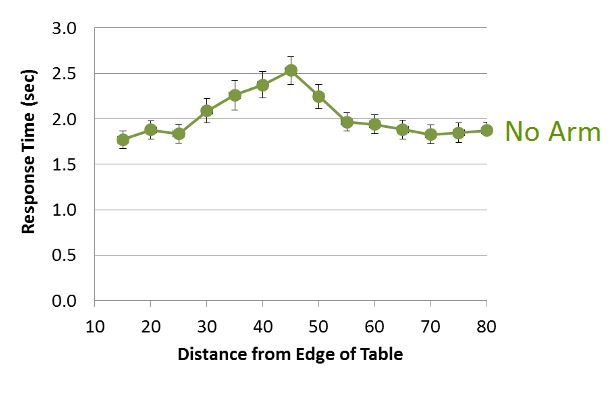
\includegraphics[width=0.75\textwidth]{no_arm_responst_time_dist}
  \caption{Response times in relation to the edge of the table in the no arm condition.} 
  \label{fig:no_arm_responst_time_dist}
\end{figure}

\begin{figure}
\centering
  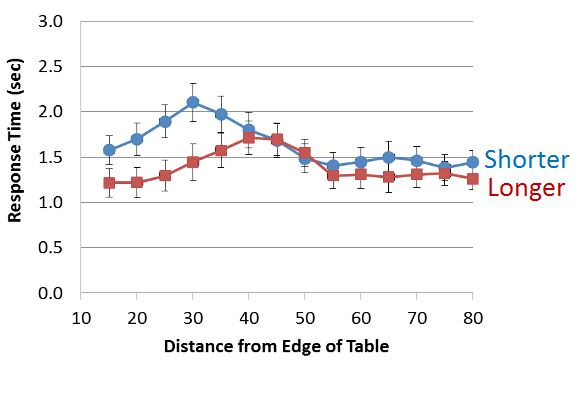
\includegraphics[width=0.75\textwidth]{short_long_arm_responst_time_dist}
  \caption{Response times in relation to the edge of the table in the shorter/longer arm condition.} 
  \label{fig:short_long_arm_responst_time_dist}
\end{figure}

\subsection{Accuracy}

In the no arm condition accuracy (crossover point) ranged from 1.15 to 0.9 . The highest estimation was at 0 degrees. The lowest estimation was at 135 degrees. (Fig. \ref{fig:no_arm_co})

\begin{figure}
\centering
  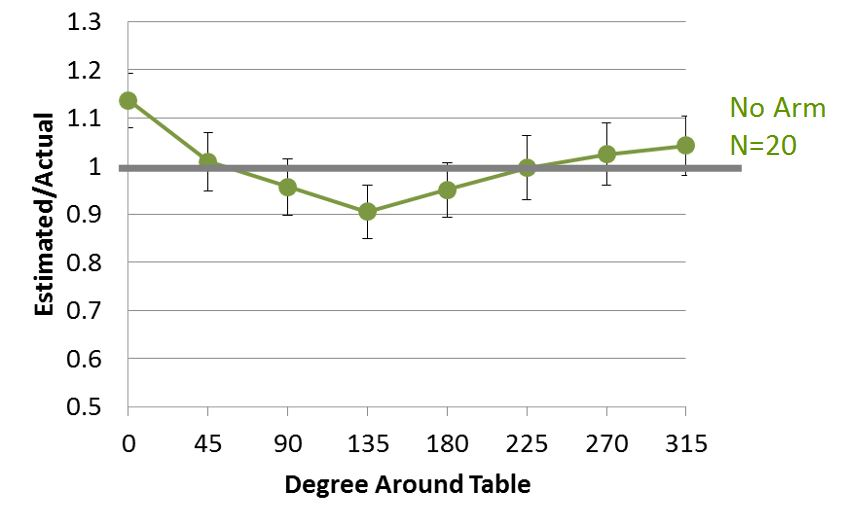
\includegraphics[width=0.75\textwidth]{no_arm_co}
  \caption{Accuracy (crossover point) of different chair angles around the table in the no arm condition} 
  \label{fig:no_arm_co}
\end{figure}

 In the shorter arm condition accuracy (crossover point) ranged from 1.1 to 0.85. The highest estimation was at 0 degrees. The lowest estimation was at 90 degrees. In the longer arm condition accuracy (crossover point) ranged from 0.66 to 0.82 . The highest estimation was at 0 degrees. The lowest estimation was at 135 degrees. (\ref{fig:short_long_arm_co}) 
 
 In all conditions the lowest estimations were between 90 to 135 degrees. This means most low estimations have occured for trials in which the ball was on the left half of the rounds table (degrees were defined clockwise around the table with 0 degrees at the participant's actual location). Since all participants were right-handed their judgments may have been less confident for trials in which the ball was in the left half of the table. 
 
 An general interaction between degree around the table and accuracy could only be found for 0 degrees, because in all conditions the estimation at 0 degrees are the highest. This is probably due to the fact that confidence is higher in the first person perspective. No significant effect could be found for the opposite position at 180 degrees. Also for all other degrees there was no significant interaction because such effects need to occur pairwise (45/215, 90/270, 135/225) which was not the case.
 
 Participants in both the shorter and longer arm condition show overall lower estimations than in the now arm condition, which is inline with the observation of reaction times. 
 

 
 \begin{figure}
\centering
  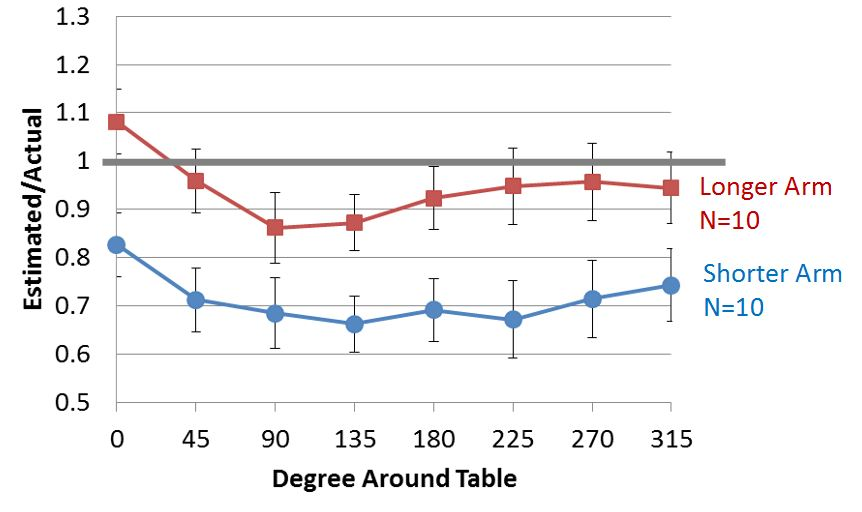
\includegraphics[width=0.75\textwidth]{short_long_arm_co}
  \caption{Accuracy (crossover point) of different chair angles around the table in the shorter/longer arm condition} 
  \label{fig:short_long_arm_co}
\end{figure}

\newpage
\clearpage
\section{Discussion}\label{discussion}

2. Follow-up: affordance judgments for others

The first follow-up experiment will be changed only in the way that participants will be asked to not imagine themselves sitting at a different location, but to judge for an avatar appearing at different locations around the table if it would be possible for him/her to reach the object. 
The main question then is if participants - after having experienced a shorter/longer virtual arm – also show an increase/decrease in estimated maximum reaching distance for the avatar. If so we would argue that temporary changes to our body not only influence how we perceive our own action capabilities but also how we perceive action capabilities of others.

3. Follow up: 3rd person adaptation

The second follow-up experiment will only change the participant’s perspective in the second part of the experiment from 1st to 3rd person perspective. This means that the participant’s own arm movements now control the arm of an avatar in the scene instead of the participant’s own virtual arm (the participant’s own arm will not be rendered at all). 
With this manipulation we want to address the question if the experience of controlling the arm of an avatar will also alter the participant’s judgement of how far he/she is able to reach. We argue that in contrast to the initial study with this manipulation the participant’s perceptual ruler is not changed and therefore expect little to no change in estimated maximum reaching distance.
\newpage
\section{Conclusion}\label{conclusion}

Need to assess strategy participants, instructions obviously not followed?

training effect

measurement accuracy of arm

80/120 vs 90/110

Based on the proposed improvements two follow up studies could provide further insights.

2. Follow-up: affordance judgments for others

The first follow-up experiment will be changed only in the way that participants will be asked to not imagine themselves sitting at a different location, but to judge for an avatar appearing at different locations around the table if it would be possible for him/her to reach the object. 
The main question then is if participants - after having experienced a shorter/longer virtual arm – also show an increase/decrease in estimated maximum reaching distance for the avatar. If so we would argue that temporary changes to our body not only influence how we perceive our own action capabilities but also how we perceive action capabilities of others.

3. Follow up: 3rd person adaptation

The second follow-up experiment will only change the participant’s perspective in the second part of the experiment from 1st to 3rd person perspective. This means that the participant’s own arm movements now control the arm of an avatar in the scene instead of the participant’s own virtual arm (the participant’s own arm will not be rendered at all). 
With this manipulation we want to address the question if the experience of controlling the arm of an avatar will also alter the participant’s judgement of how far he/she is able to reach. We argue that in contrast to the initial study with this manipulation the participant’s perceptual ruler is not changed and therefore expect little to no change in estimated maximum reaching distance.

\onecolumn
% einfacher Zeilenabstand
\singlespacing
% Literaturliste soll im Inhaltsverzeichnis auftauchen
\newpage
\addcontentsline{toc}{section}{Bibliography}
% Literaturverzeichnis anzeigen
\renewcommand\refname{Bibliography}
\bibliographystyle{plainnat}
\bibliography{Hauptdatei}

%% Index soll Stichwortverzeichnis heissen
% \newpage
% % Stichwortverzeichnis soll im Inhaltsverzeichnis auftauchen
% \addcontentsline{toc}{section}{Stichwortverzeichnis}
% \renewcommand{\indexname}{Stichwortverzeichnis}
% % Stichwortverzeichnis endgueltig anzeigen
% \printindex

\onehalfspacing
% evtl. Anhang

% Eidesstattliche Erklärung
\section*{}
\thispagestyle{empty}

\begin{verbatim}

\end{verbatim}

\begin{LARGE}Eidesstattliche Erklärung zur Masterarbeit\end{LARGE}
\begin{verbatim}


\end{verbatim}
Ich versichere, die von mir vorgelegte Arbeit selbstständig verfasst zu haben. Alle Stellen, die wörtlich oder sinngemäß aus veröffentlichten oder nicht veröffentlichten Arbeiten anderer entnommen sind, habe ich als entnommen kenntlich gemacht. Sämtliche Quellen und Hilfsmittel, die ich für die Arbeit benutzt habe, sind angegeben. Die Arbeit hat mit gleichem Inhalt bzw. in wesentlichen Teilen noch keiner anderen Prüfungsbehörde vorgelegen.



\begin{displaymath}
% use packages: array
\begin{array}{ll}
Unterschrift:~~~~~~~~~~~~~~~~~~~~~~~~~~~~~~~~~~~~~~~~~~
& Ort, Datum:~~~~~~~~~~~~~~~~~~~~~~~~~~~~~~~~~~~~~~~~~~
\end{array}
\end{displaymath}


\end{document}